\documentclass[tikz,border=10pt]{article}
\newcommand{\course}{Physics}
\usepackage[margin=1.5in]{geometry}
\newcommand{\instructor}{Athan Zhang \& Jeffrey Chen}
\usepackage{amsmath}
\usepackage{pgfplots}
\pgfplotsset{width=10cm, compat=1.9}
\usepackage[inline]{enumitem}
\pgfplotsset{compat=1.12}


% Document Body
\begin{document}

% Title
\begin{center}
\textbf{\Huge Problem Set 01} % Replace "#" with the problem set number
\end{center}

% Course and Instructor Information
\begin{flushleft}
\emph{Course:} \course \\
\emph{Instructors:} \instructor \\
\end{flushleft}

% Problem 1
\section*{Problem 1}

An electron in a television tube travels the 16-cm distance from the grid to the screen at an average speed of $4 \times 10^{7} \text{m/s}$.
\begin{enumerate}
    \item How long does the trip take?
    \item It now travels at a speed of $4 \times 10^{5} \text{m/s}$. How long does it take now?
\end{enumerate}

% Problem 2
\section*{Problem 2}
Cupid fires an arrow that strikes Jeffrey, producing the usual sounds of harp music and bird chirping as Jeffrey falls in love with a frog. If Cupid heard these tell-tale sounds exactly 3.2 seconds after firing the arrow, and the average speed of the arrow was 40 m/s, what was the distance separating them? Assume the speed of sound to be 340 m/s.

% Problem 3
\section*{Problem 3}

The height of a certain projectile is related to time by $y = -5(t -5)^{2} + 125$ where $y$ is in meters and $t$ is in seconds.

\begin{enumerate}
    \item Sketch $y$ versus $t$ for $0 \leq t \leq 10$s
    \item Find the average velocity for each of the 2-s time intervals between the given time interval. Then sketch $v_{avg}$ versus $t$
    \item Find the instantaneous velocity as a function of time.
\end{enumerate}

% Problem 4
\section*{Problem 4}

A ball is thrown straight up. What is the velocity of the ball at the top of its flight? What is the acceleration at that point?

% Problem 5
\section*{Problem 5}

An object projected up with initial velocity $v$ attains a height $H$. Another object projected up with initial velocity $2v$ will attain what height with respect to $H$?

% Problem 6
\section*{Problem 6}

At which of the following points is the velocity of the particle at a minimum?

\begin{center}
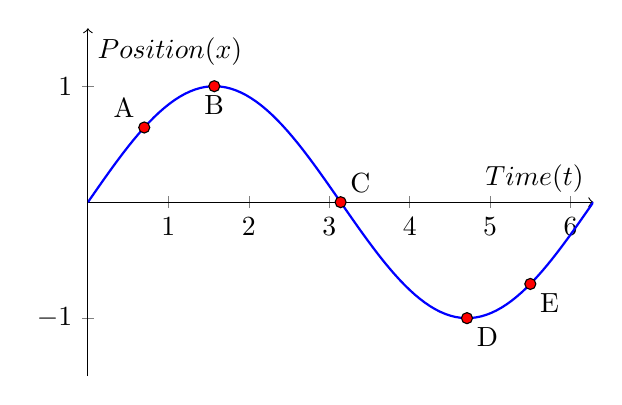
\begin{tikzpicture}
  \begin{axis}[
    height=6cm,
    width=8cm,
    xlabel=$Time (t)$,
    ylabel=$Position (x)$,
    xmin=0, xmax=2*pi,
    ymin=-1.5, ymax=1.5,
    axis lines=middle,
    axis line style={->},
    samples=100,
    domain=0:2*pi
  ]

  % Plot sine curve
  \addplot[blue, thick] {sin(deg(x))};

  % Points A-E
  \coordinate (A) at (.7, 0.644);
  \draw[fill=red] (A) circle[radius=2pt] node[above left] {A};

  \coordinate (B) at (pi/2, 1);
  \draw[fill=red] (B) circle[radius=2pt] node[below] {B};

  \coordinate (C) at (pi, 0);
  \draw[fill=red] (C) circle[radius=2pt] node[above right] {C};

  \coordinate (D) at (3*pi/2, -1);
  \draw[fill=red] (D) circle[radius=2pt] node[below right] {D};

  \coordinate (E) at (5.5, -0.705);
  \draw[fill=red] (E) circle[radius=2pt] node[below right] {E};

  \end{axis}
\end{tikzpicture}
\end{center}

% Problem 7
\section*{Problem 7}

If a ball is tossed up with an initial speed of 2.0 m/s, does it spend more time in the top 0.1 m of the toss or the bottom 0.1 m of the toss? (Assume $g = 9.8\;\text{m/s}^{2}$)

\end{document}
